% 
% Lecture Template for ME3023 -  Measurements in Mechanical Systems - Tennessee Technological University
%
% Spring 2020 - Summer 2020
% Tristan Hill, May 07, 2020 - June 12, 2020 - July 08, 2020
% Module 6->4 - Steady State Circuits
% Topic 1 - Components, Units, and Symbols
%
% Lecture Template for ME3023 -  Measurements in Mechanical Systems - Tennessee Technological University
% Spring 2020 - Summer 2020 - Fall 2020 - Spring 2021 - Summer 2021
% Tristan Hill, May 07, 2020 - June 12, 2020 - July 08, 2020 - Novemeber 02, 2020 - March 28, 2021 - May 25, 2021
% Module Name: To Err is Human
% Topic 1 - Accuracy and Error

\documentclass[fleqn]{beamer} % for presentation (has nav buttons at bottom)

\usepackage{/home/thill/Documents/lectures/measurements_lectures/measurements_lectures}

\author{ME3023 - Measurements in Mechanical Systems} 

\newcommand{\MNUM}{4\hspace{2mm}} % Module number
\newcommand{\TNUM}{1\hspace{2mm}} % Topic number 
\newcommand{\moduletitle}{Steady State Circuits}
\newcommand{\topictitle}{Components, Units, and Symbols} 

\newcommand{\sectiontitleI}{Common Passive Components}
\newcommand{\sectiontitleII}{Important Electrical Quantities}
\newcommand{\sectiontitleIII}{Units and Symbols}
\newcommand{\sectiontitleIV}{Types of Switches}

% custom box
\newsavebox{\mybox}

\title{Lecture Module - \moduletitle}

\date{Mechanical Engineering\vspc Tennessee Technological University}

\begin{document}
	
	\lstset{language=MATLAB,basicstyle=\ttfamily\small,showstringspaces=false}
	
	\frame{\titlepage \center\begin{framed}\Large \textbf{Topic \TNUM - \topictitle}\end{framed} \vspace{5mm}}


% Section 0: Outline
\frame{
\large \textbf{Topic \TNUM - \topictitle} \vspace{3mm}\\

\begin{itemize}

	\item \sectiontitleI    \vspc % Section I
	\item \sectiontitleII 	\vspc % Section II
	\item \sectiontitleIII 	\vspc %Section III
	\item \sectiontitleIV 	\vspc %Section IV

\end{itemize}

}

% Section I:
\section{\sectiontitleI}

% Section I - Frame I:
\frame{
\frametitle{\sectiontitleI}
%\small
Passive components affect the behavior of a circuit in different ways but they do   not generate power and can only absorb energy or transform it into heat. Active components on the other hand...

\begin{itemize}
\item Resistor 
\item Capacitor
\item Inductor
\end{itemize}

Most circuits require an active power source for operation. A voltage source is used in most applications however current sources are also available and are needed for specialized electrical applications. 

}


% Section I - Frame II:
\frame{
\frametitle{\sectiontitleI}

Components are identified by color codes and numbering systems. However it is always a good idea to measure for yourself because a marking can be  incorrect  or a component may be damaged. \vspc

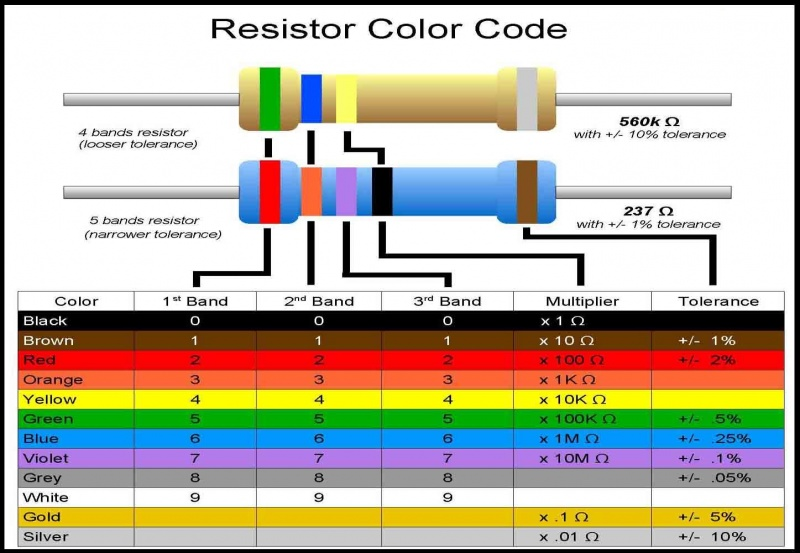
\includegraphics[scale=.25]{resistor_color_codes.jpg}
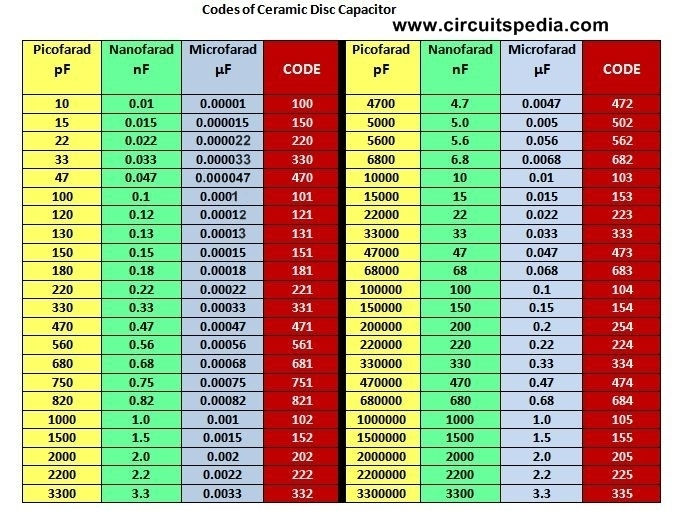
\includegraphics[scale=.3]{ceramic_capacitor_codes.jpg}

}


% Section II:
\section{\sectiontitleII}

% Section II - Frame I:
\frame{
\frametitle{\sectiontitleII}

\begin{itemize}

	\begin{multicols}{2}
	\item {\BL \hspcu} - the physical property of matter that causes it to experience a force when placed in an electromagnetic field.
	
	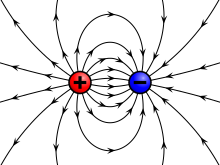
\includegraphics[scale=.5]{charges_plus_minus.png}
	\end{multicols}
	
	\item {\PR \hspcu} - the difference in electric potential between two points ... can be caused by electric charge, by electric current through a magnetic field, by time-varying magnetic fields, or some combination of these three.
	
	\item {\RD \hspcu} - the rate of flow of electric charge past a point or region. An electric current is said to exist when there is a net flow of electric charge through a region.

\end{itemize}

}


% Section II - Frame II:
\frame{
\frametitle{\sectiontitleII}

\begin{itemize}


	\item {\BL \hspcu} - a measure of a components opposition to the flow of electric current. The inverse quantity is electrical conductance, and is the ease with which an electric current passes.  
	
	
	\item {\PR \hspcu} - the ratio of the change in electric charge of a system to the corresponding change in its electric potential (voltage).
	
	\item {\RD \hspcu} - the tendency of an electrical conductor to oppose a change in the electric current flowing through it. The flow of electric current creates a magnetic field around the conductor. The field strength depends on the magnitude of the current, and follows any changes in current.

\end{itemize}

}


% Section III:
\section{\sectiontitleIII}

% Section III - Frame I:
\frame{\small
\frametitle{\sectiontitleIII}
	
	\renewcommand{\arraystretch}{1.2}
	\begin{tabular}{|c|c|c|c|} \hline
		Quantity & Symbol & Unit & Abbr. \\ \hline\hline
	    Charge & Q,q & Coulomb & C \\ \hline
	    Voltage & V,v & Volt & v\\ \hline
	    Current & I,i & Ampere & A \\ \hline
	    Resistance & R & Ohm & $\Omega$ \\ \hline
	    Capacitance & C & Farad & F \\ \hline
	    Inductance & L & Henry & H  \\ \hline
	\end{tabular}
	
	\vspace*{10mm} Question: When should you use upper case or lower case letters for electrical quantities?

}

% Section III - Frame II:
\frame{\small
\frametitle{\sectiontitleIII}
	
	When working with a or building a circuit  you need a diagram. Draw or find one before you begin. Here are some commonly used symbols.\vspccc
	
	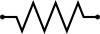
\includegraphics[scale=.4]{resistor_symbol.png} \hspace{15mm}
	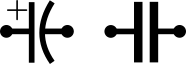
\includegraphics[scale=.4]{capacitor_symbol.png} \hspace{15mm}
	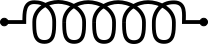
\includegraphics[scale=.4]{inductor_symbol.png} \vspace{10mm}
	
	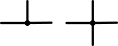
\includegraphics[scale=.5]{node_symbol.png} \hspace{15mm}
	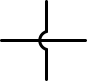
\includegraphics[scale=.5]{jump_symbol.png} \hspace{15mm}
	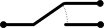
\includegraphics[scale=.5]{switch_symbol.png} \hspace{15mm}
	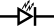
\includegraphics[scale=.7]{led_symbol.png} \hspace{15mm}

}

%% Section IV:
\section{\sectiontitleIV}

% Section IV - Frame I:
\frame{
\frametitle{\sectiontitleIV}
\small


A switch is a mechanical-electrical device that that can change from a continuous state to a dis-continuous state and they are used as a mechanical interface to a circuit. There many different types of switches for different purposes and this is not an exhaustive list.

\begin{itemize}
\item Toggle Switches
\item Momentary Switches
\item Reed Switches
\item Level or Float Switches
\item and many more
\end{itemize}

}
	
% Section IV - Frame II:
\frame{
\frametitle{\sectiontitleIV}
\small

Toggle switches are are possibly the most commonly used switches and they come in many different forms.\vspace{5mm}\\

	{\bf Poles } - \vspace{5mm}\\
	
	{\bf Throws} -  \vspace{5mm}\\
	
	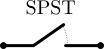
\includegraphics[scale=.7]{spst_symbol.png} \hspace{5mm} 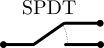
\includegraphics[scale=.7]{spdt_symbol.png} \hspace{5mm}
	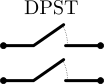
\includegraphics[scale=.7]{dpst_symbol.png} \hspace{5mm} 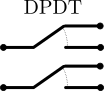
\includegraphics[scale=.7]{dpdt_symbol.png}
}
 



\end{document}





